\clearpage
\section{Testy, wyniki i wnioski}		%5

W rozdziale przedstawiono sposób sprawdzenia działania aplikacji oraz wnioski wynikające z testów. Testy miały charakter funkcjonalny i wydajnościowy. Ich celem było potwierdzenie, że system poprawnie obsługuje wiele źródeł obrazu, rozpoznaje osoby, zapisuje zdarzenia oraz pozwala dobrać model do możliwości sprzętu.

\subsection{Zakres testów}

Testy obejmowały następujące obszary:

\begin{itemize}
\item uruchomienie aplikacji i wczytanie konfiguracji,
\item dodawanie wielu źródeł wideo,
\item wykrywanie osób na obrazie,
\item działanie trybu dziennego i klasyfikacji ubioru,
\item działanie masek ignorowanych obszarów,
\item zapis klipów zdarzeń po przekroczeniu minimalnego czasu widoczności,
\item filtrowanie i podgląd zapisanych zdarzeń,
\item zmianę modelu YOLO z poziomu aplikacji,
\item porównanie obciążenia sprzętu dla różnych wariantów modelu.
\end{itemize}

\subsection{Test wielu źródeł obrazu}

Aplikację sprawdzono na kilku jednoczesnych źródłach wideo. System poprawnie prezentował obraz w siatce, aktualizował metryki FPS oraz nanosił ramki detekcji na osoby widoczne w kadrze. W trybie dziennym osoby niespełniające wzorca ubioru były oznaczane jako intruzi, natomiast osoby zgodne ze wzorcem mogły zostać oznaczone jako pracownicy. Przykład testu wielu źródeł przedstawiono na rysunku \ref{fig:test-wiele-zrodel}.

\begin{figure}[H]
\centering
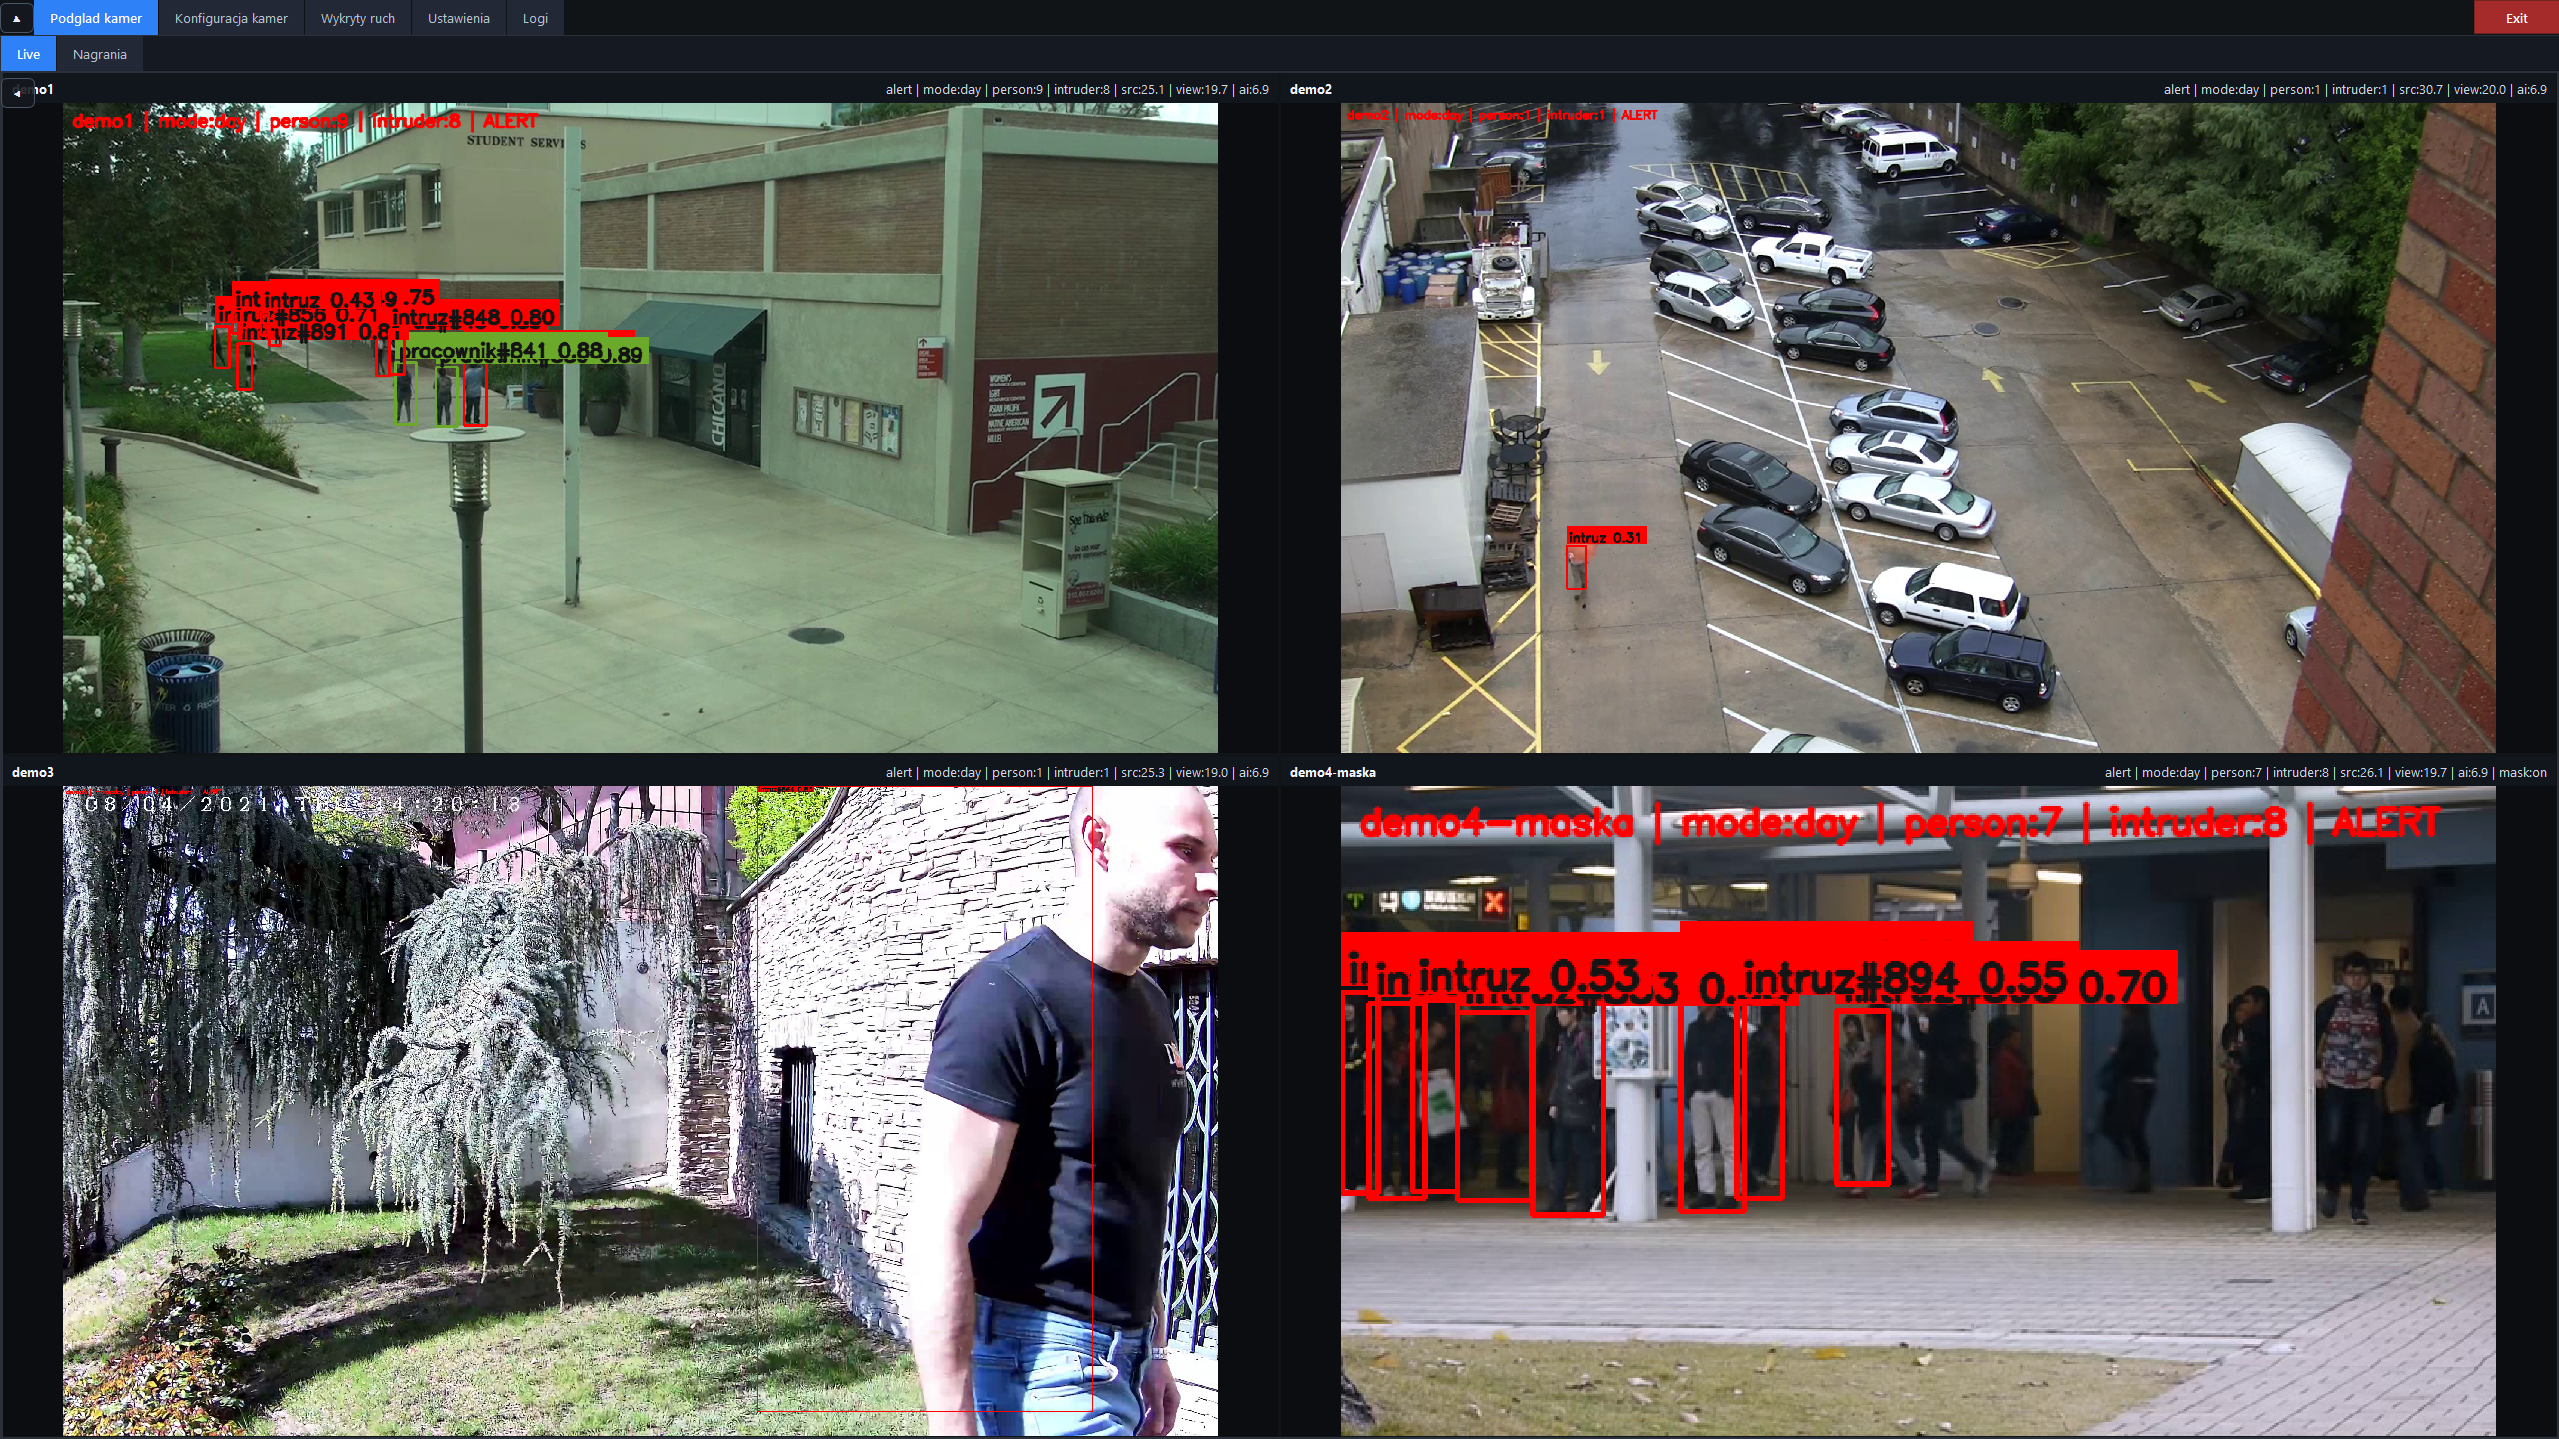
\includegraphics[width=0.95\textwidth]{rys/działanie-kamer-2.png}
\caption{Test pracy systemu na wielu źródłach obrazu.}
\label{fig:test-wiele-zrodel}
\end{figure}

\subsection{Test trybu dziennego, wzorca ubioru i masek}

Tryb dzienny wykorzystuje model segmentacyjny do wyznaczenia maski sylwetki. Na podstawie tej maski aplikacja pobiera kolory ubioru i porównuje je z ustawionym wzorcem. Testy potwierdziły, że takie podejście pozwala ograniczyć wpływ tła na analizę koloru. W jednym ze scenariuszy zmieniono wzorzec stroju pracownika na czarną górną część ubioru oraz niebieskawe spodnie, co pokazano na rysunku \ref{fig:test-zmiana-wzorca}. Po zastosowaniu tej konfiguracji system poprawnie rozpoznał osobę spełniającą nowy wzorzec jako pracownika, co przedstawia rysunek \ref{fig:test-zmiana-ustawien}. Funkcja masek ignorowanych obszarów pozwoliła dodatkowo wykluczyć fragmenty kadru, które nie powinny brać udziału w detekcji.

\begin{figure}[H]
\centering
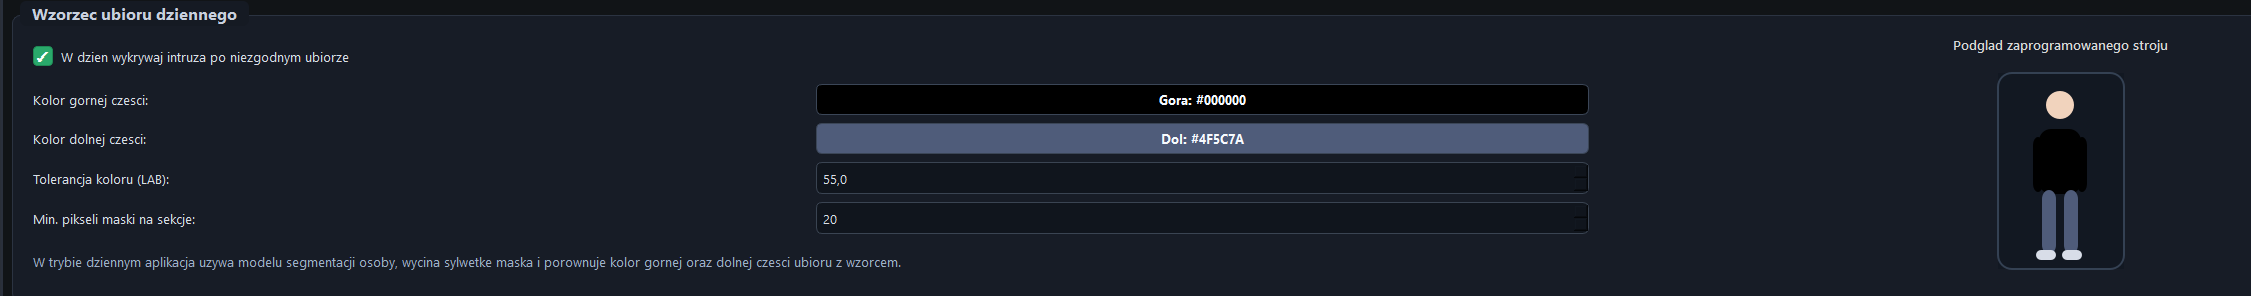
\includegraphics[width=0.95\textwidth]{rys/po-zmianie-wykladu-ustawienia.png}
\caption{Ustawienie wzorca ubioru dziennego na czarną górę i niebieskawe spodnie.}
\label{fig:test-zmiana-wzorca}
\end{figure}

\begin{figure}[H]
\centering
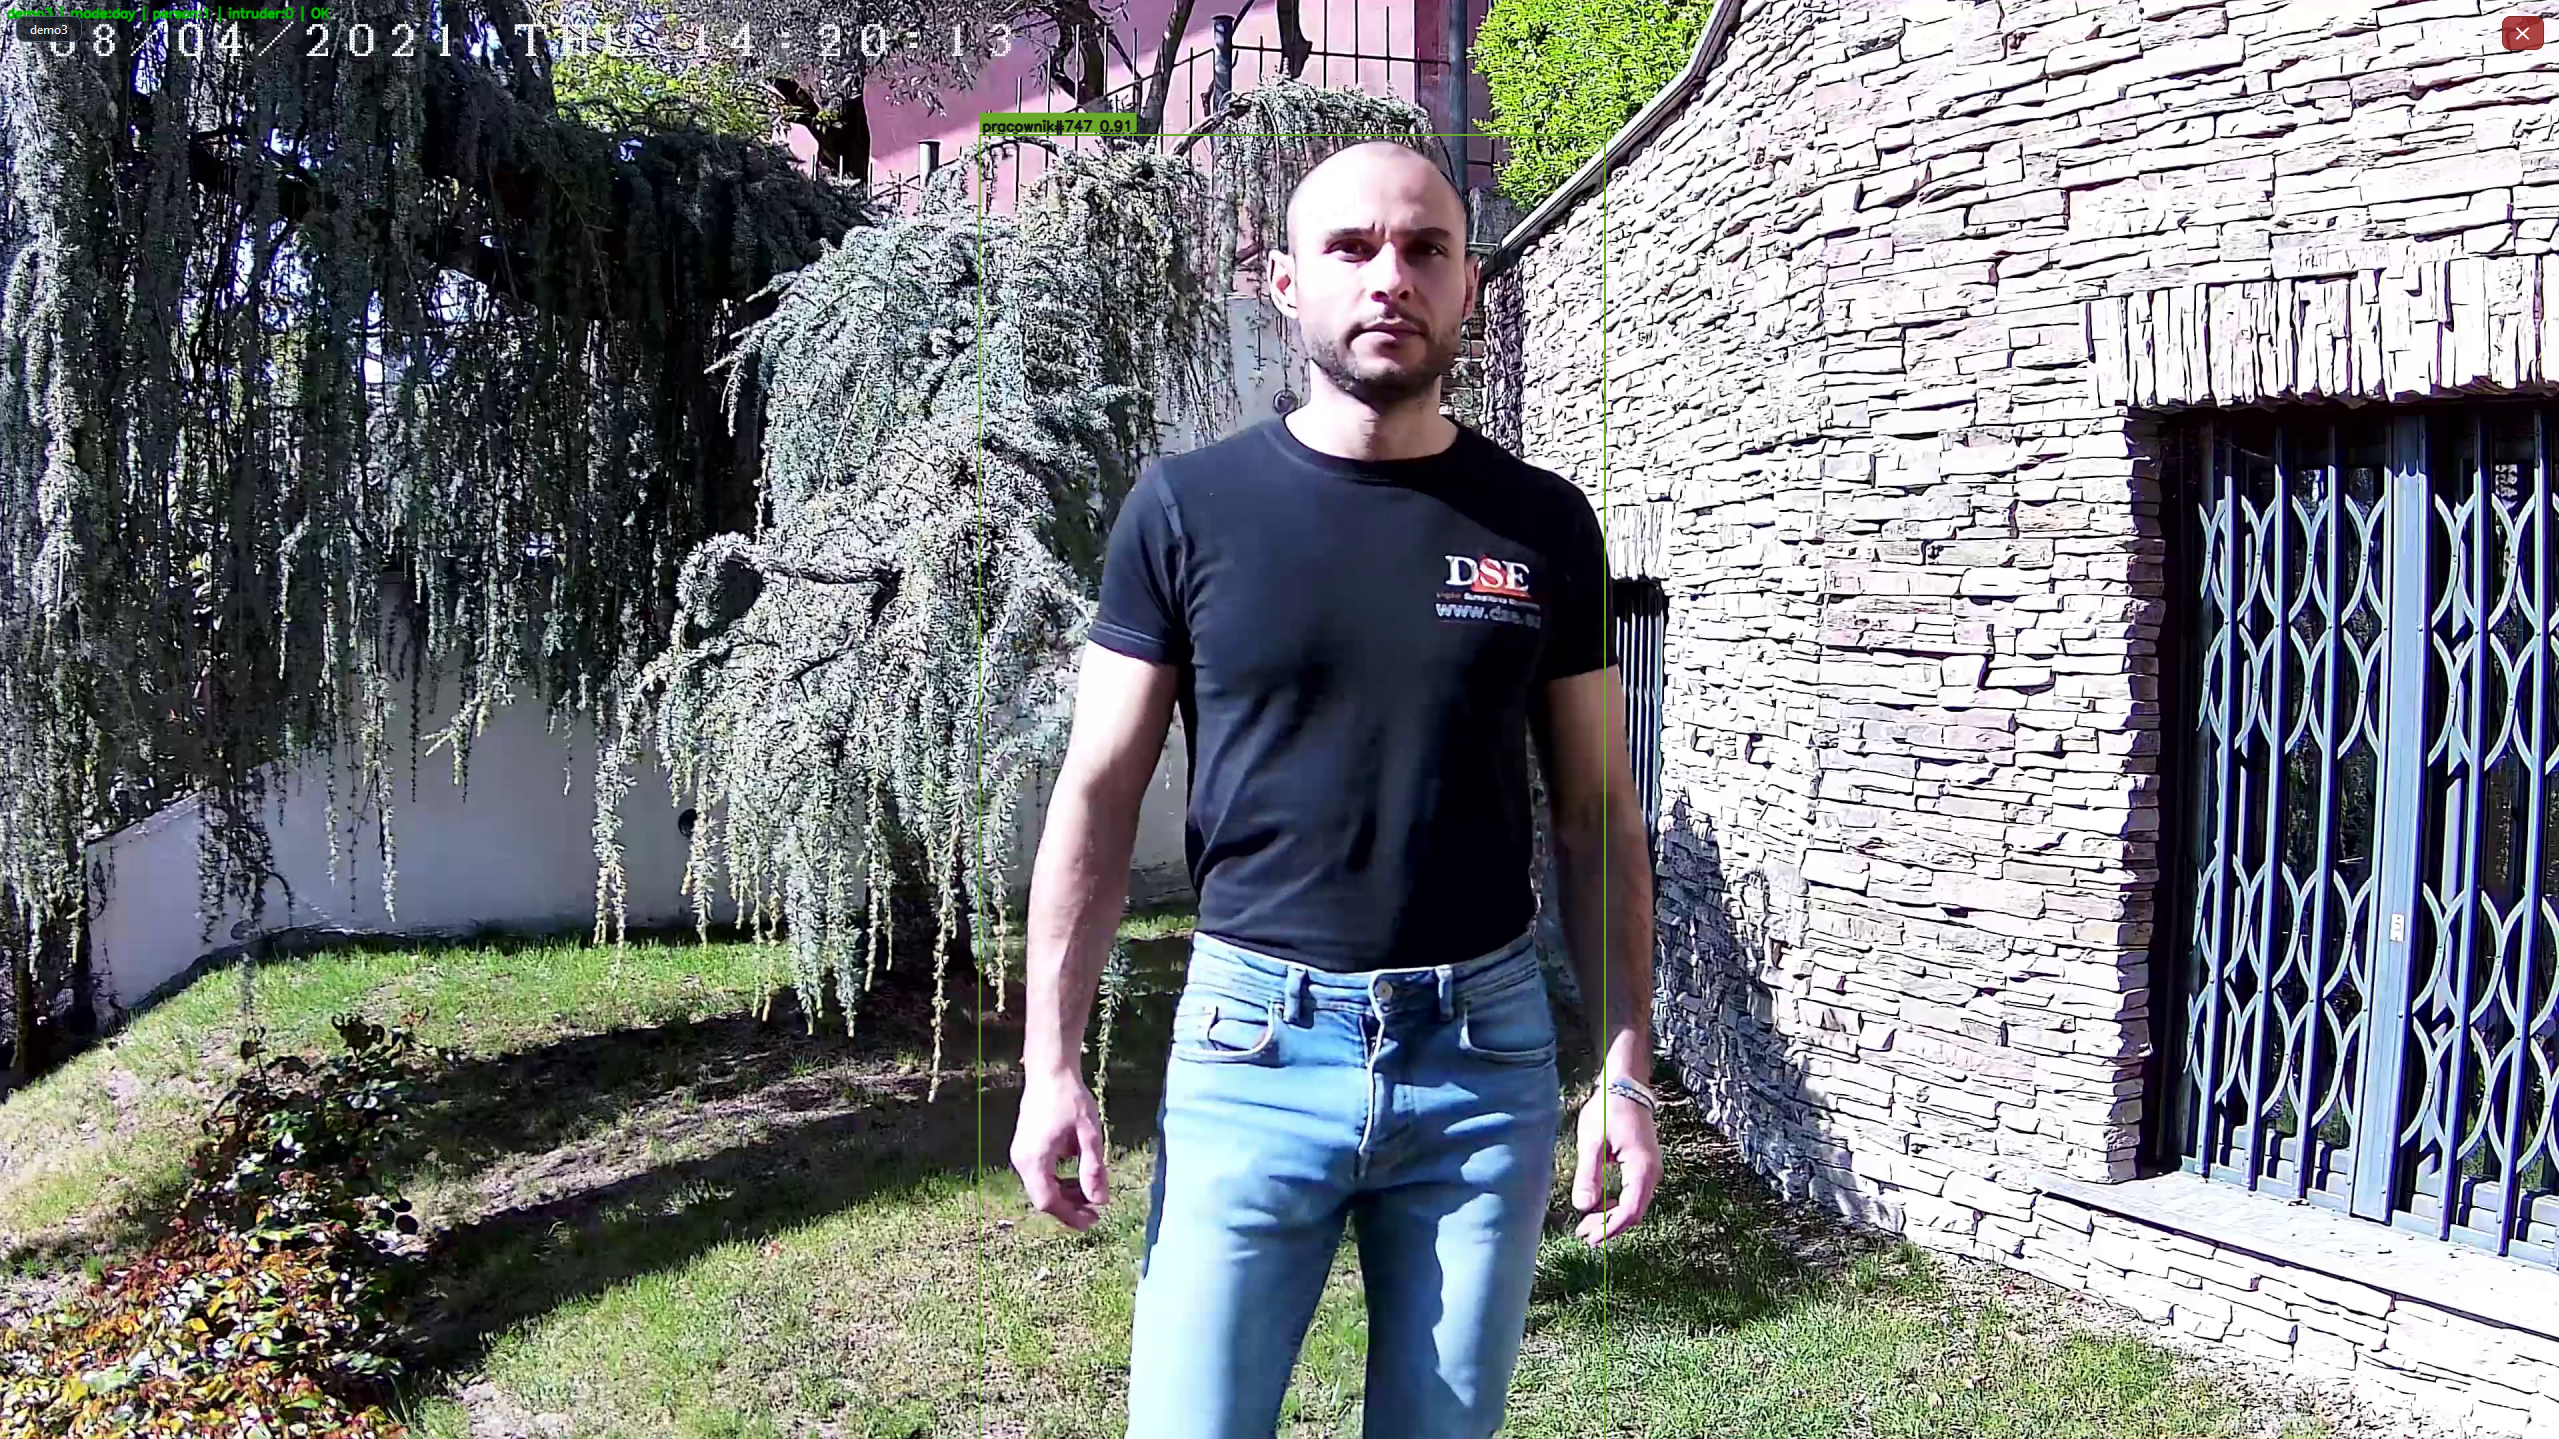
\includegraphics[width=0.95\textwidth]{rys/po-zmianie-wykladu-kamera.png}
\caption{Poprawna klasyfikacja osoby jako pracownika po zmianie wzorca ubioru.}
\label{fig:test-zmiana-ustawien}
\end{figure}

\subsection{Test archiwizacji zdarzeń}

Podczas testów system zapisywał klipy zdarzeń po spełnieniu warunku minimalnego czasu widoczności osoby. W zakładce \textit{Wykryty ruch} możliwe było filtrowanie wpisów według okresu, kamery, trybu pracy oraz godzin. Wybranie wpisu powodowało załadowanie podglądu zapisanego materiału, a przycisk otwarcia pliku pozwalał przejść do materiału źródłowego.

Istotnym elementem jest limit \texttt{max\_saved\_events}. Po przekroczeniu tego limitu system usuwa najstarsze wpisy i odpowiadające im pliki, dzięki czemu katalog zdarzeń nie rośnie bez kontroli.

\subsection{Porównanie modeli i obciążenia sprzętu}

Aplikacja pozwala łatwo porównywać różne warianty modeli YOLO. Domyślnym kompromisem jest profil \textit{medium}, który łączy akceptowalną dokładność z rozsądnym obciążeniem sprzętu. Model nano został przetestowany jako lżejsza alternatywa dla standardowego modelu. Konfigurację z włączonym modelem nano pokazano na rysunku \ref{fig:nano-ustawienia}. W tym wariancie system nadal obsługuje kilka źródeł obrazu i wykonuje detekcję osób, co przedstawia rysunek \ref{fig:nano-kamery}. Jednocześnie, ze względu na mniejszy model, użycie GPU jest wyraźnie niższe niż przy większych wariantach YOLO. Pomiar obciążenia CPU i GPU podczas pracy modelu nano przedstawiono na rysunku \ref{fig:nano-wydajnosc}.

\begin{figure}[H]
\centering
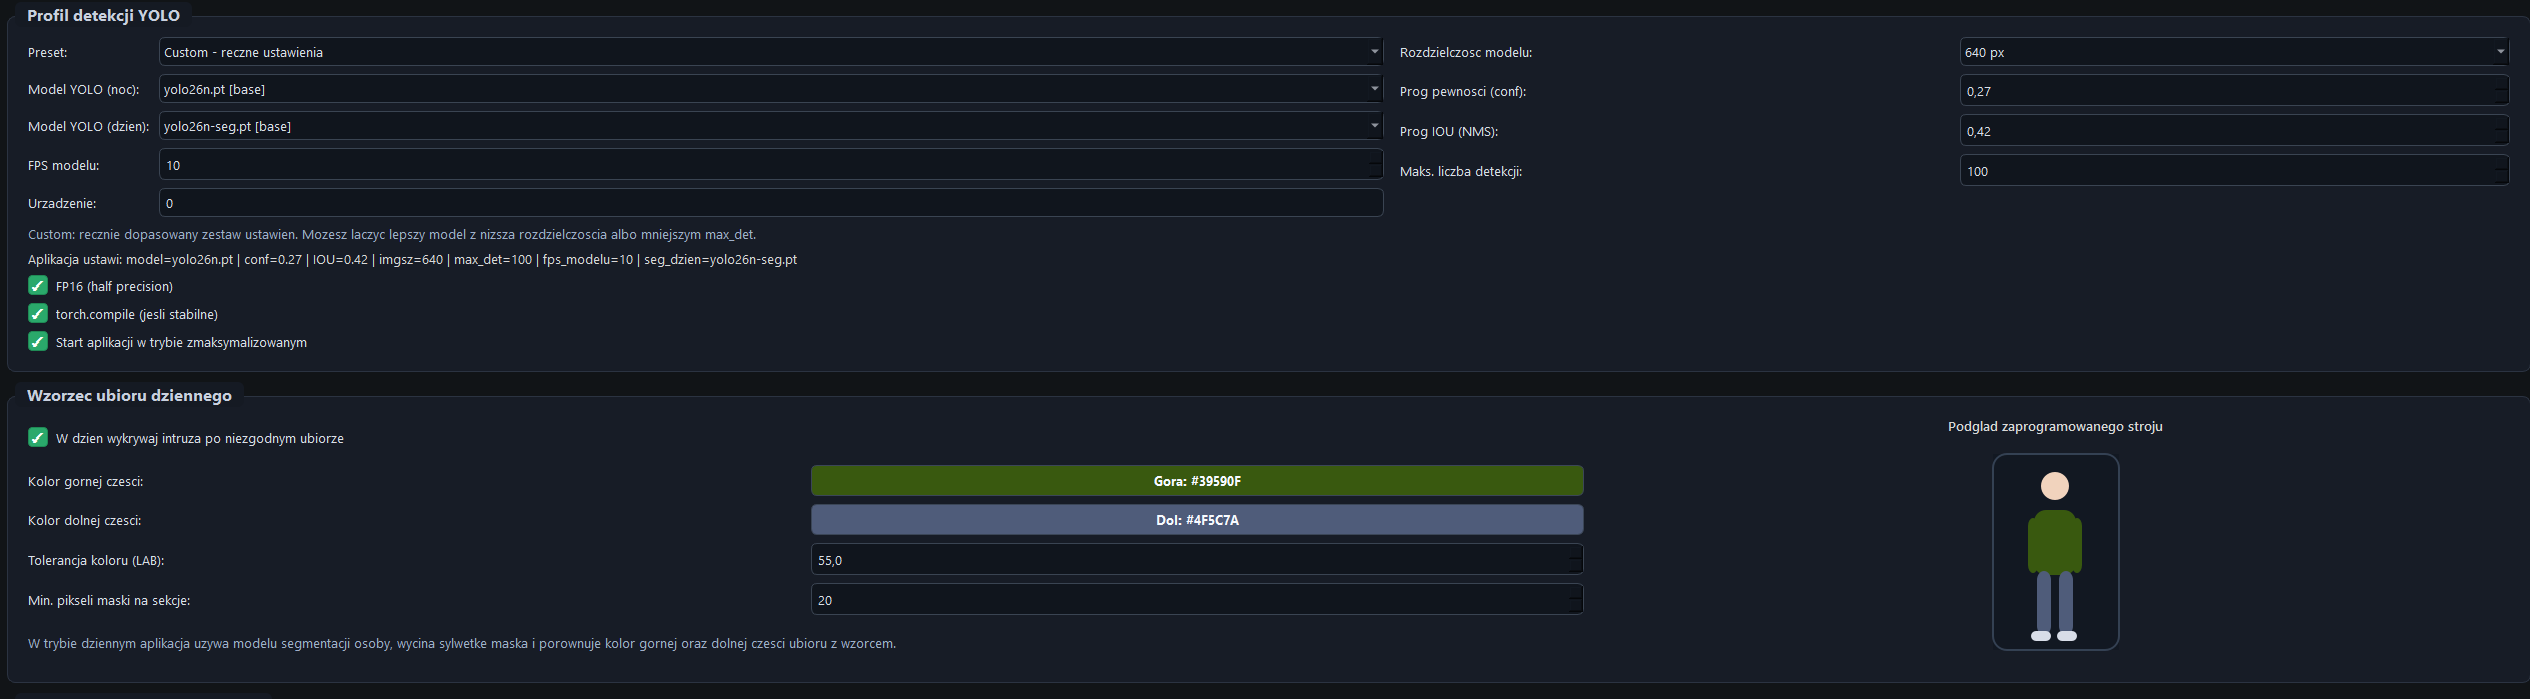
\includegraphics[width=0.95\textwidth]{rys/nano-model-ustawienia.png}
\caption{Włączony model nano w ustawieniach aplikacji.}
\label{fig:nano-ustawienia}
\end{figure}

\begin{figure}[H]
\centering
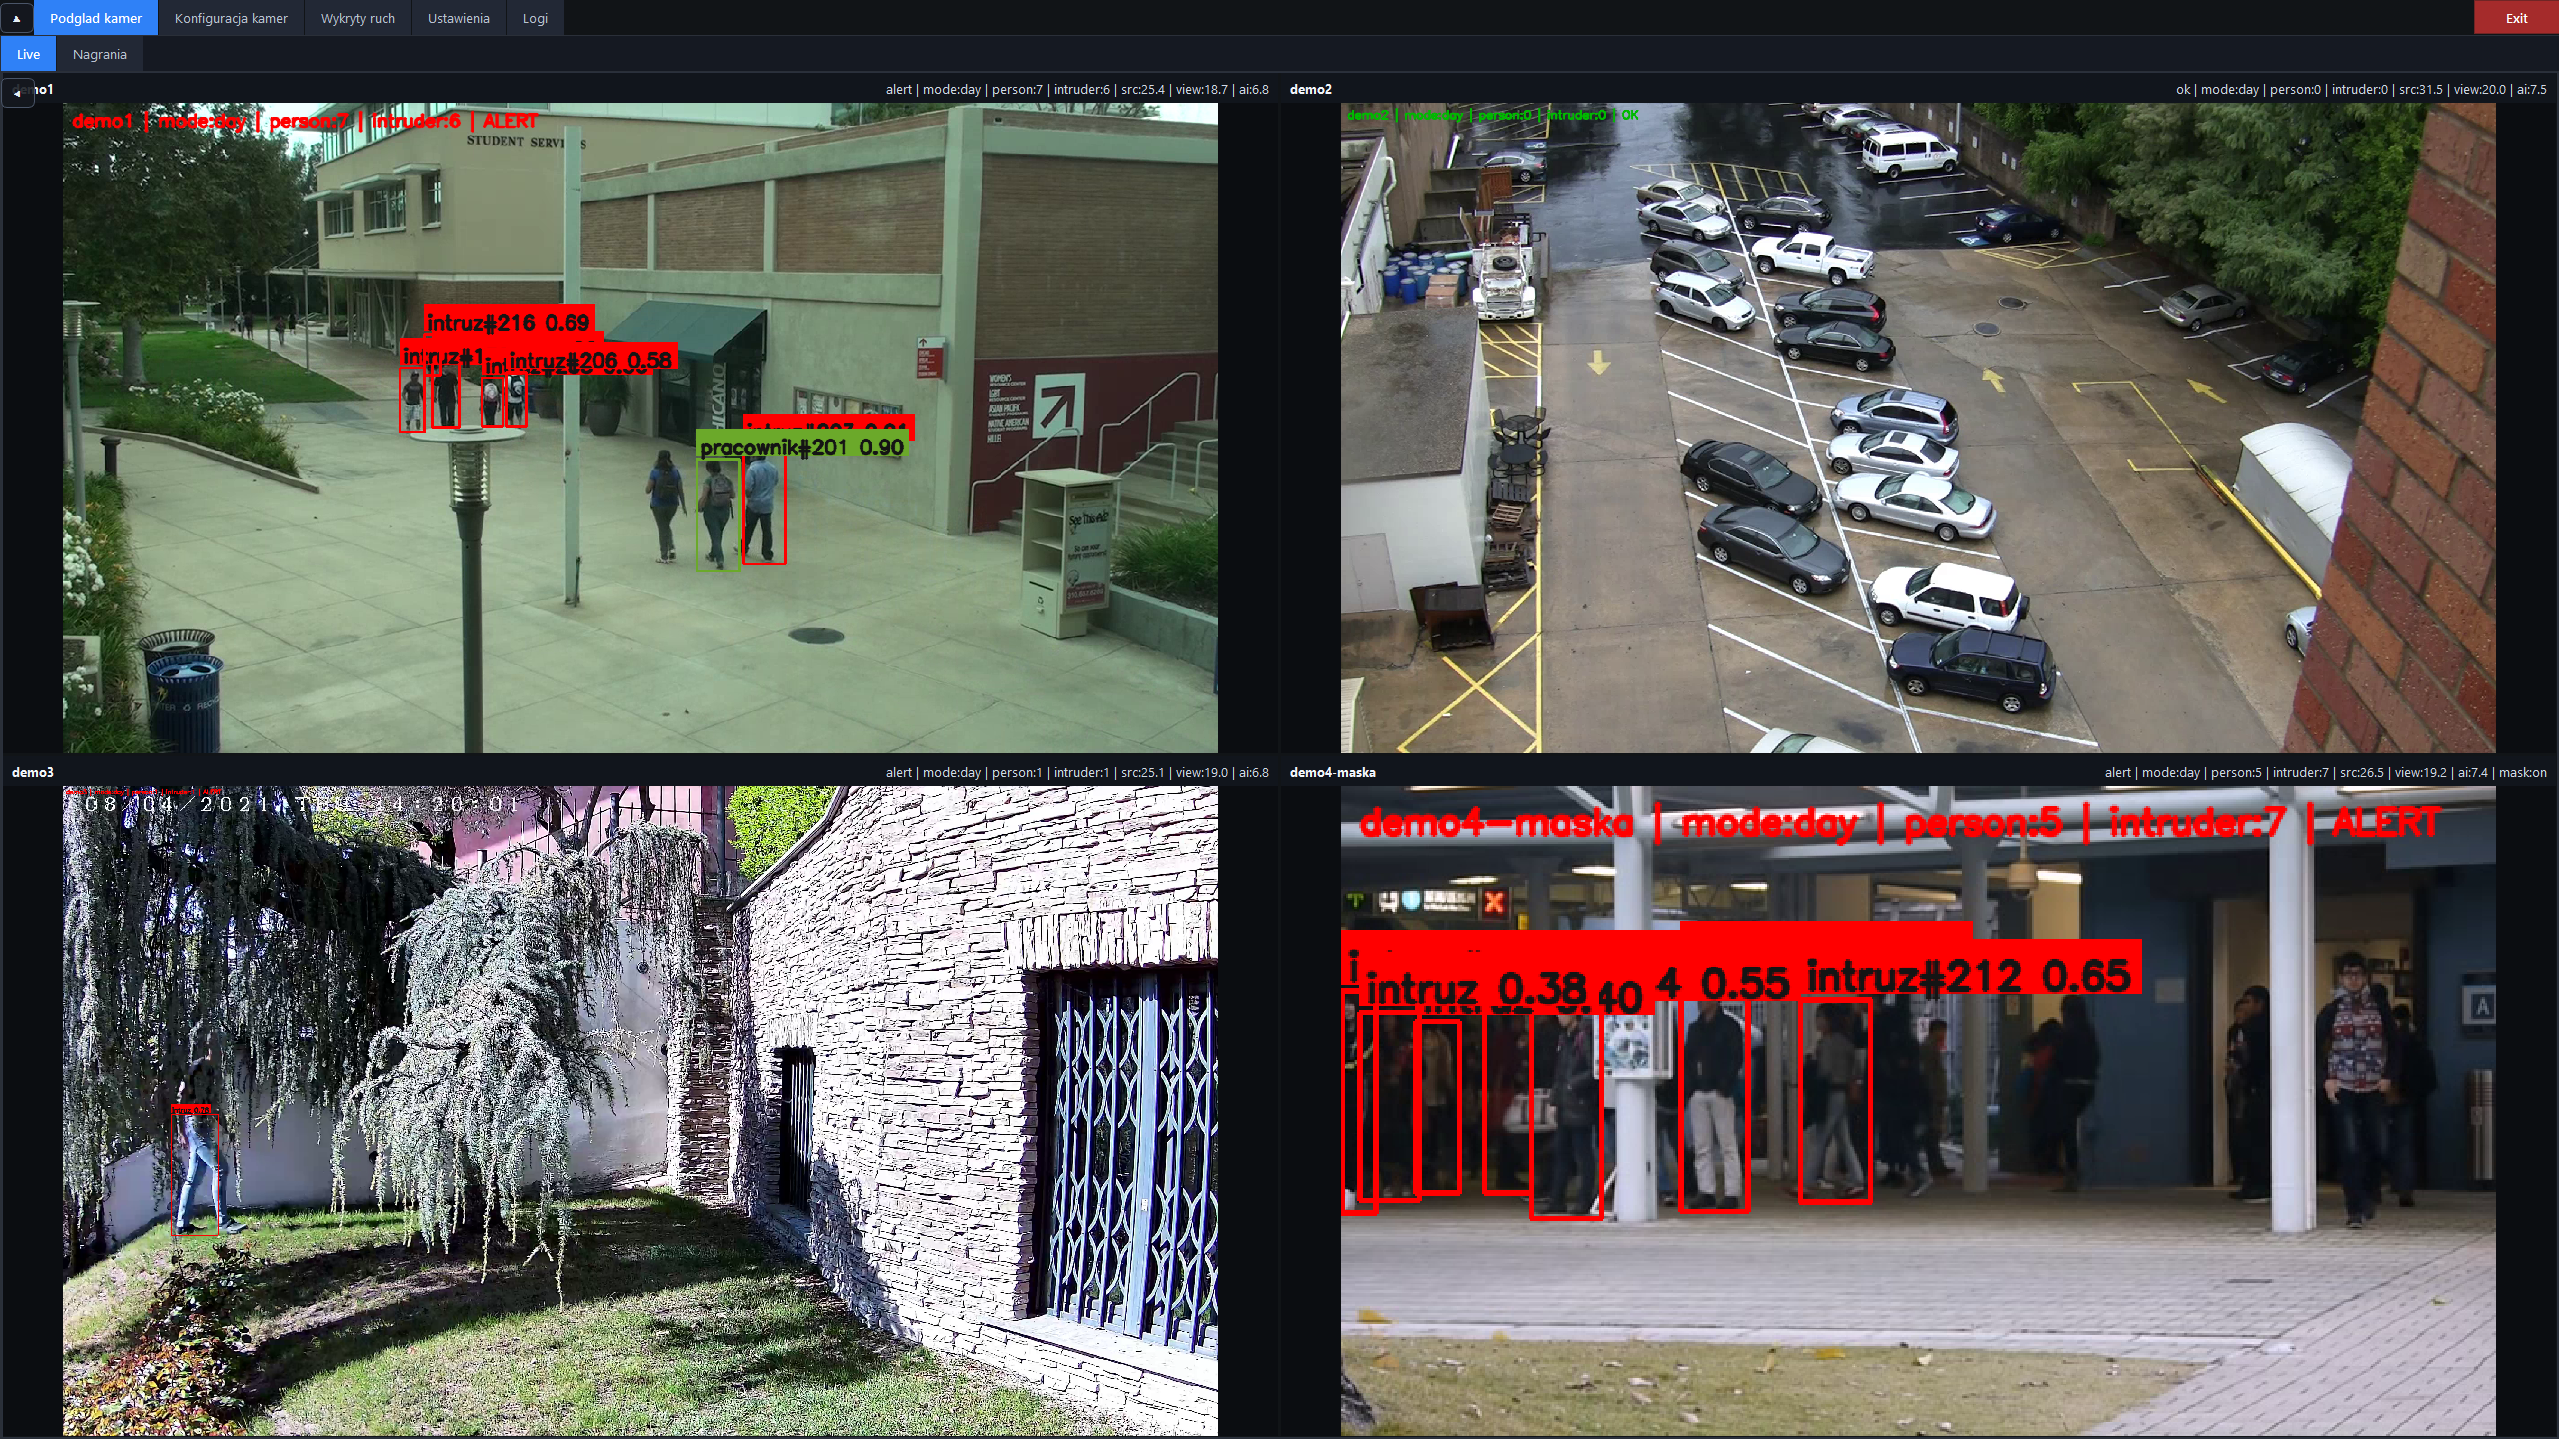
\includegraphics[width=0.95\textwidth]{rys/nano-model-kamery.png}
\caption{Działanie systemu na wielu źródłach obrazu po przełączeniu na model nano.}
\label{fig:nano-kamery}
\end{figure}

\begin{figure}[H]
\centering
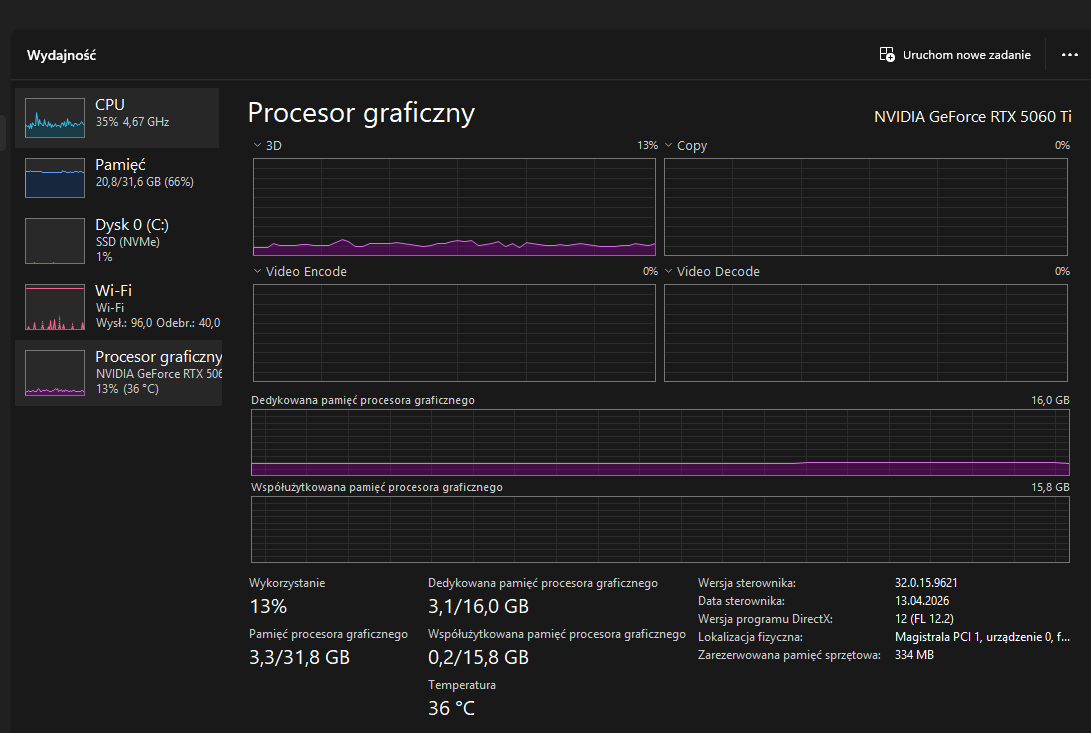
\includegraphics[width=0.95\textwidth]{rys/nano-model-cpuGpu-usage.png}
\caption{Pomiar użycia CPU i GPU podczas pracy na modelu nano, pokazujący niższe obciążenie GPU niż przy większym modelu.}
\label{fig:nano-wydajnosc}
\end{figure}

Dla większych modeli i wyższych rozdzielczości inferencji zaobserwowano wyższe obciążenie GPU oraz CPU. Jest to oczekiwane, ponieważ model analizuje większy obraz i wykonuje więcej operacji. Przykład takiego pomiaru pokazano na rysunku \ref{fig:wysokie-ustawienia}. W praktycznym wdrożeniu wybór modelu powinien zależeć od liczby kamer, jakości obrazu, wymaganego poziomu dokładności oraz dostępnego sprzętu.

\begin{figure}[H]
\centering
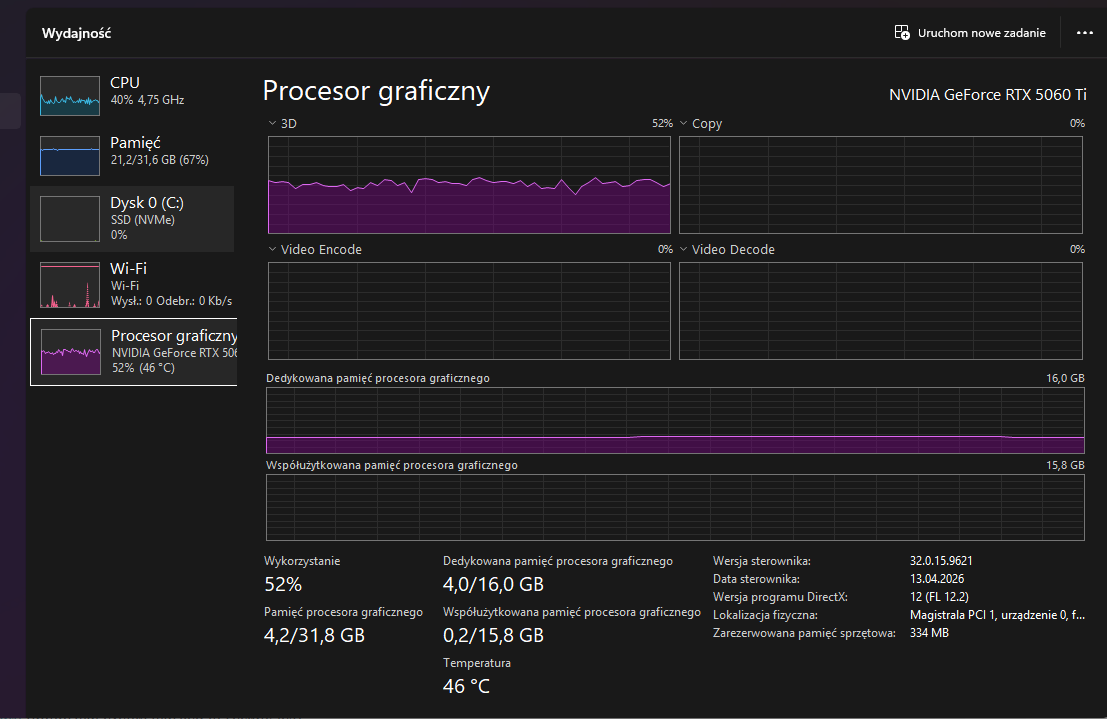
\includegraphics[width=0.95\textwidth]{rys/użycie-cpuGpu-na-wysokich-ustawieniach-wykrywania.png}
\caption{Przykład większego obciążenia sprzętu przy wysokich ustawieniach detekcji.}
\label{fig:wysokie-ustawienia}
\end{figure}

\subsection{Wnioski}

Zrealizowany system spełnia założenia projektu. Aplikacja umożliwia pracę na wielu źródłach obrazu, wykrywanie osób, klasyfikację intruzów w trybie dziennym i nocnym, zapis zdarzeń oraz przegląd historii wykryć. Interfejs graficzny pozwala operatorowi zarządzać kamerami, modelami i ustawieniami bez konieczności znajomości kodu.

Najważniejsze zalety systemu to:

\begin{itemize}
\item możliwość obsługi wielu źródeł obrazu w jednym oknie,
\item rozdzielenie trybu dziennego i nocnego,
\item wykorzystanie segmentacji do analizy ubioru pracowników,
\item wygodna konfiguracja modeli i progów detekcji z poziomu GUI,
\item automatyczny zapis klipów zdarzeń z możliwością filtrowania,
\item możliwość porównywania modeli pod kątem wydajności i dokładności.
\end{itemize}

Do dalszego rozwoju można zaliczyć integrację z powiadomieniami zewnętrznymi, rozbudowę raportów, dodanie kont użytkowników, szyfrowanie zapisanych materiałów oraz dokładniejszą analizę zachowania osób w monitorowanej przestrzeni.
